\section{Method}
This section explains how the implementation was done and how the experiments were conducted. After that follows an outline of the experiment setup and a motivation for the designs of the experiments.
\subsection{Implementation}
The implemented word predictor had three basic components: N-grams with probability smoothing, grammar constraints and context recognition. The implementation was done using two NLP-libraries and several books to make a corpus. KYLM\footnote{A full list of resources can be found in section \ref{sec:resources}} was a library capable of producing N-grams with different smoothing techniques. We used it to process our corpus and make an ARPA-file, consisting of N-grams of different sizes and their probability derived from the corpus and chosen smoothing technique. We also used OpenNLP for POS (Part-of-Speech) tagging that was used in the implementation of grammar constraints and context recognition. The rest of the program: searching through the N-grams, grammar constraints, context recognition and user interface was implemented by the authors. The core method of choosing the words to be predicted was to compare large N-grams, choose the grams with highest probabilities, and if more words were required, fall back to smaller grams.

\paragraph{Grammar constraints}
The implemented grammar constraints worked by removing predictions that could be considered very unlikely to be grammatically correct.

The implemented grammar constraints with ideas of why they should work were:

\begin{itemize}
	\item Avoid repeated words - When the user has entered a word it should be highly unlikely that the same word would appear directly after it.
	\item Avoid multiple conjunctions -  A user rarely wants to enter several conjunctions into a single sentence, for example several “and”s. Therefore only a few conjunctions are allowed.
	\item Avoid verbs in succession - An English sentence rarely has several verbs in succession. By using POS tagging, even verbs not in the corpus can be identified and more accurate predictions can be made after that verb.
	\item Ensure SVO - Ensures SVO (Subject-Verb-Object) order for personal pronouns, meaning that only appropriate word types are predicted after a personal pronoun. The allowed word types are verbs, modal verbs, adverbs and conjunctions.
	\item Possessive pronoun + adjective/noun - A possessive pronoun (my/her/his/its) is often followed by either an adjective or a noun, so any other word type is ignored.
\end{itemize}

\paragraph{Context recognition}
Context recognition was implemented by exchanging the word “it” with the first noun of the sentence, together with any possessive pronoun or determiner. For example, the sentence “my dog is nice and it is…” would be changed to “my dog is nice and my dog is…”. The word “it” will often point to the subject of the sentence.

For some sentences the first occurring noun is not the subject but rather the object, for example in the sentence “I like the dog because it is...”. However, the implemented context recognition will work well even for sentences like this, because the first noun was “dog”, which in fact was what “it” referred to.

The word “it” is not replaced when predicting the word directly after “it”, since it could sometimes make predictions grammatically incorrect.

\subsection{Evaluation}

\begin{figure}[t]
\center
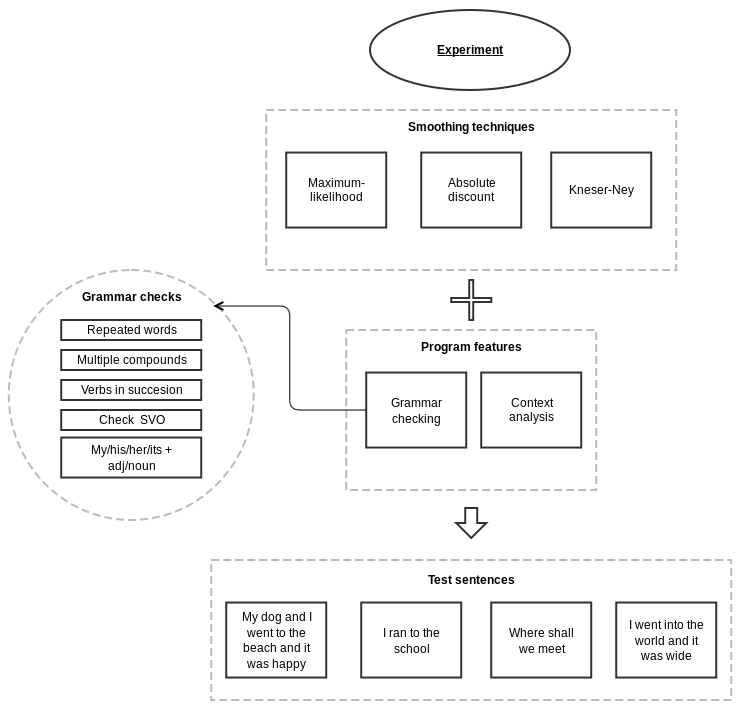
\includegraphics[width=0.7\textwidth]{img/experiment_diagram.png}
\caption{Diagram showing how experiments were generated}
\label{fig:experiments}
\end{figure}

To test our hypotheses, a qualitative inductive method was used. Evaluation and comparison of the different functionalities was made by measuring keystroke rates for typing whole sentences. This was a widely used method for similar projects\cite{keystrokes}, and suited our project as it is an objective performance evaluation, compared to perception testing which produces more subjective results.

In the constructed keystroke experiment, for a given word, the number of keystrokes were the number of letters that the participant had to enter in order for the word predictor to suggest the word the participant meant to write. In this experiment, the word predictor might suggest the thought of word without any keystrokes, in which case the keystroke count for that word is zero. Spaces between words did not count as keystrokes.

The process of generating experiments is shown in figure \ref{fig:experiments}. Four sentences that were thought to display the differences in the different functionalities were constructed. Tests were then performed for each sentence, for each combination of functionalities and for each smoothing technique, which made a total of 48 different tests. After that, some tests were rerun with case-insensitivity. POS tagging did not work well with case insensitivity so grammar constraints were therefore always set to \emph{off}, resulting in an additional 24 tests.

\paragraph{Test sentences}
The motivation for the test sentences and their anticipated results were:

\emph{My dog and I went to the beach and it was happy}
This sentence was constructed to test the context functionality of the word predictor. It contains the noun “dog” which is the subject of the sentence. With context recognition, the word “it” will be replaced by “my dog” which should make the predicted words more accurate and thus save more keystrokes.

\emph{I ran to the school}
This sentence was constructed to test the grammar functionality. The sentence contains “I”, a personal pronoun, for which some grammar constraints are implemented. Some improbable suggestions could therefore be removed which should result in a higher probability of showing the correct word, and thus less keystrokes should be required.

\emph{I went into the world and it was wide}
This sentence was fabricated to show the context recognition for when the word “it” refers to the object of the sentence, “the world”. Since “the world was wide” exists as an N-gram in the corpus, and “it was wide” is not a very common statement compared to other “it was”-combinations, this should result in more accurate word predictions.

The sentence also tests grammar constraints in a similar manner as the sentence “I ran to the school”.

\emph{Where shall we meet}
This sentence was constructed as an everyday language sentence, for showing how the word predictor could perform for text messaging. Context recognition will not matter for this sentence, but grammar constraints could make the predictions more accurate.

\subsubsection{Experimental setup}
\paragraph{Corpus}
The corpus used in the experiments consisted of 10 books\footnote{The full list of books can be found in section \ref{sec:resources}} of varying themes and content, downloaded from \url{http://www.gutenberg.org/}. Choosing the books was done at random but from different categories such as children's books, science fiction and philosophy.

The corpus was manipulated by removing citation marks, underscores and new lines. Periods, commas and question marks were made into separate words by adding a space before them. The case-insensitive corpus was the same corpus but with only lowercase letter.

\paragraph{N-gram size}
A maximum N-gram size of 4 was chosen for the experiments. Having a larger N-gram size was deemed to not give a significant increase in performance compared to the exponentially increasing number of N-grams and computation time. Grams of a higher size than 5 was also considered being too dependent on the corpus which could result in the word predictor generating very unlikely predictions.